\section{Trabalhos correlacionados}

Existem muitos trabalhos com tratamento de dados de acelerômetro para reconhecimento
de padrões de movimento.
 Dentre eles o artigo \emph{Deep Learning for Sensor-based Activity Recognition}\cite*[]{DeepLearningSensorBasedActivitie}
Onde vemos sobre as diferentes abordagem no métodos utilizados convencionalmente. Onde os dados são adquiridos e a partir
deles é realizado uma engenharia de características para abstrair informações de alto nível com alto grau de separabilidade.
E após isso implementar um algoritmo de reconhecimento de padrões convencional. Esse método pode ser visto na figura 1.

\begin{figure}[H]
    \center
    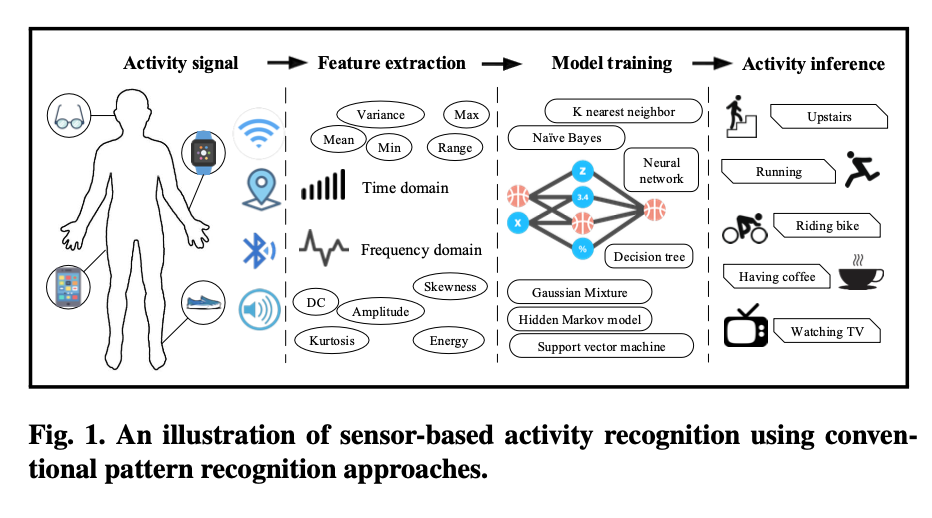
\includegraphics[width=8cm]{images/conventional}
\end{figure}

Já na abordagem de Deep Learning os dados são utilizados para treinamento de uma rede neural artificial de várias camadas e grande dimensão.
Dessa forma os dados podem servir de input diretamente do sensor e a rede convolucional de neurônios vai ajustar os pesos de suas funções de ativação
na direção que otimiza a classificação. Podemos ver esse procedimento na figura 2.

\begin{figure}[H]
    \center
    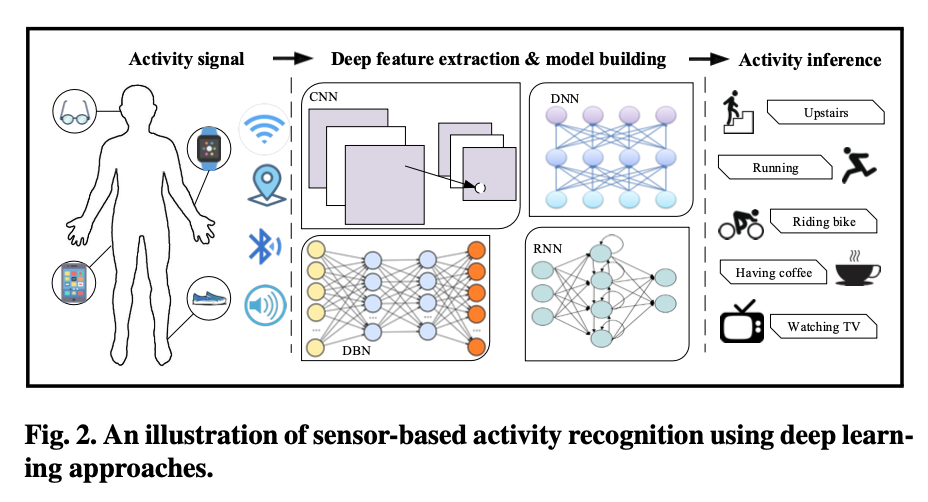
\includegraphics[width=8cm]{images/deeplearning}
\end{figure}



Outro artigo que retrata do assunto foi escrito pelo professor Leonardo Torres da UFMG \emph{Novel approaches to human activity recognition based on accelerometer data}\cite*[]{HumanRecognitionLeonardoTorres}.


Também realizei pesquisas de projetos sobre o assunto. Um muito próximo é o chamado Magic Wand. Um clássico
exemplo do framework de deep learning para microcontroladores Tensor Flow Lite.\footcite[]{TensorFlow Lite: https://www.tensorflow.org/lite}
Nesse exemplo há o uso dos dados de um sensor acelerômetro para identificar movimentos atribuídos à ele.
